\documentclass{article}
\usepackage[utf8x]{inputenc}
\usepackage{ucs}
\usepackage{amsmath} 
\usepackage{amsfonts}
\usepackage{upgreek}
\usepackage[english,russian]{babel}
\usepackage{graphicx}
\usepackage{float}
\usepackage{textcomp}
\usepackage{hyperref}
\usepackage{mathtools}
\usepackage{geometry}
  \geometry{left=2cm}
  \geometry{right=1.5cm}
  \geometry{top=1cm}
  \geometry{bottom=2cm}
\usepackage{tikz}
\usepackage{ccaption}
\usepackage{multicol}
%\setlength{\columnsep}{1.5cm}
%\setlength{\columnseprule}{0.2pt}
\usepackage{listings}

\DeclarePairedDelimiter\ceil{\lceil}{\rceil}
\DeclarePairedDelimiter\floor{\lfloor}{\rfloor}

\begin{document}
\pagenumbering{gobble}

\lstset{
  language=C,                % choose the language of the code
  basicstyle=\linespread{1.1}\ttfamily,
  columns=fixed,
  fontadjust=true,
  basewidth=0.5em,
  keywordstyle=\color{blue}\bfseries,
  commentstyle=\color{gray},
  stringstyle=\ttfamily\color{orange!50!black},
  showstringspaces=false,
  %numbers=false,                   % where to put the line-numbers
  numbersep=5pt,
  numberstyle=\tiny\color{black},
  numberfirstline=true,
  stepnumber=1,                   % the step between two line-numbers.        
  numbersep=10pt,                  % how far the line-numbers are from the code
  backgroundcolor=\color{white},  % choose the background color. You must add \usepackage{color}
  showstringspaces=false,         % underline spaces within strings
  captionpos=b,                   % sets the caption-position to bottom
  breaklines=true,                % sets automatic line breaking
  breakatwhitespace=true,         % sets if automatic breaks should only happen at whitespace
  xleftmargin=.2in,
  extendedchars=\true,
  keepspaces = true,
}
\lstset{literate=%
   *{0}{{{\color{red!20!violet}0}}}1
    {1}{{{\color{red!20!violet}1}}}1
    {2}{{{\color{red!20!violet}2}}}1
    {3}{{{\color{red!20!violet}3}}}1
    {4}{{{\color{red!20!violet}4}}}1
    {5}{{{\color{red!20!violet}5}}}1
    {6}{{{\color{red!20!violet}6}}}1
    {7}{{{\color{red!20!violet}7}}}1
    {8}{{{\color{red!20!violet}8}}}1
    {9}{{{\color{red!20!violet}9}}}1
}

\setlength{\columnseprule}{0.4pt}


\title{Семинар \#14: Деревья.\vspace{-5ex}}\date{}\maketitle

\section*{Часть 1: Бинарные деревья поиска} 

\begin{center}
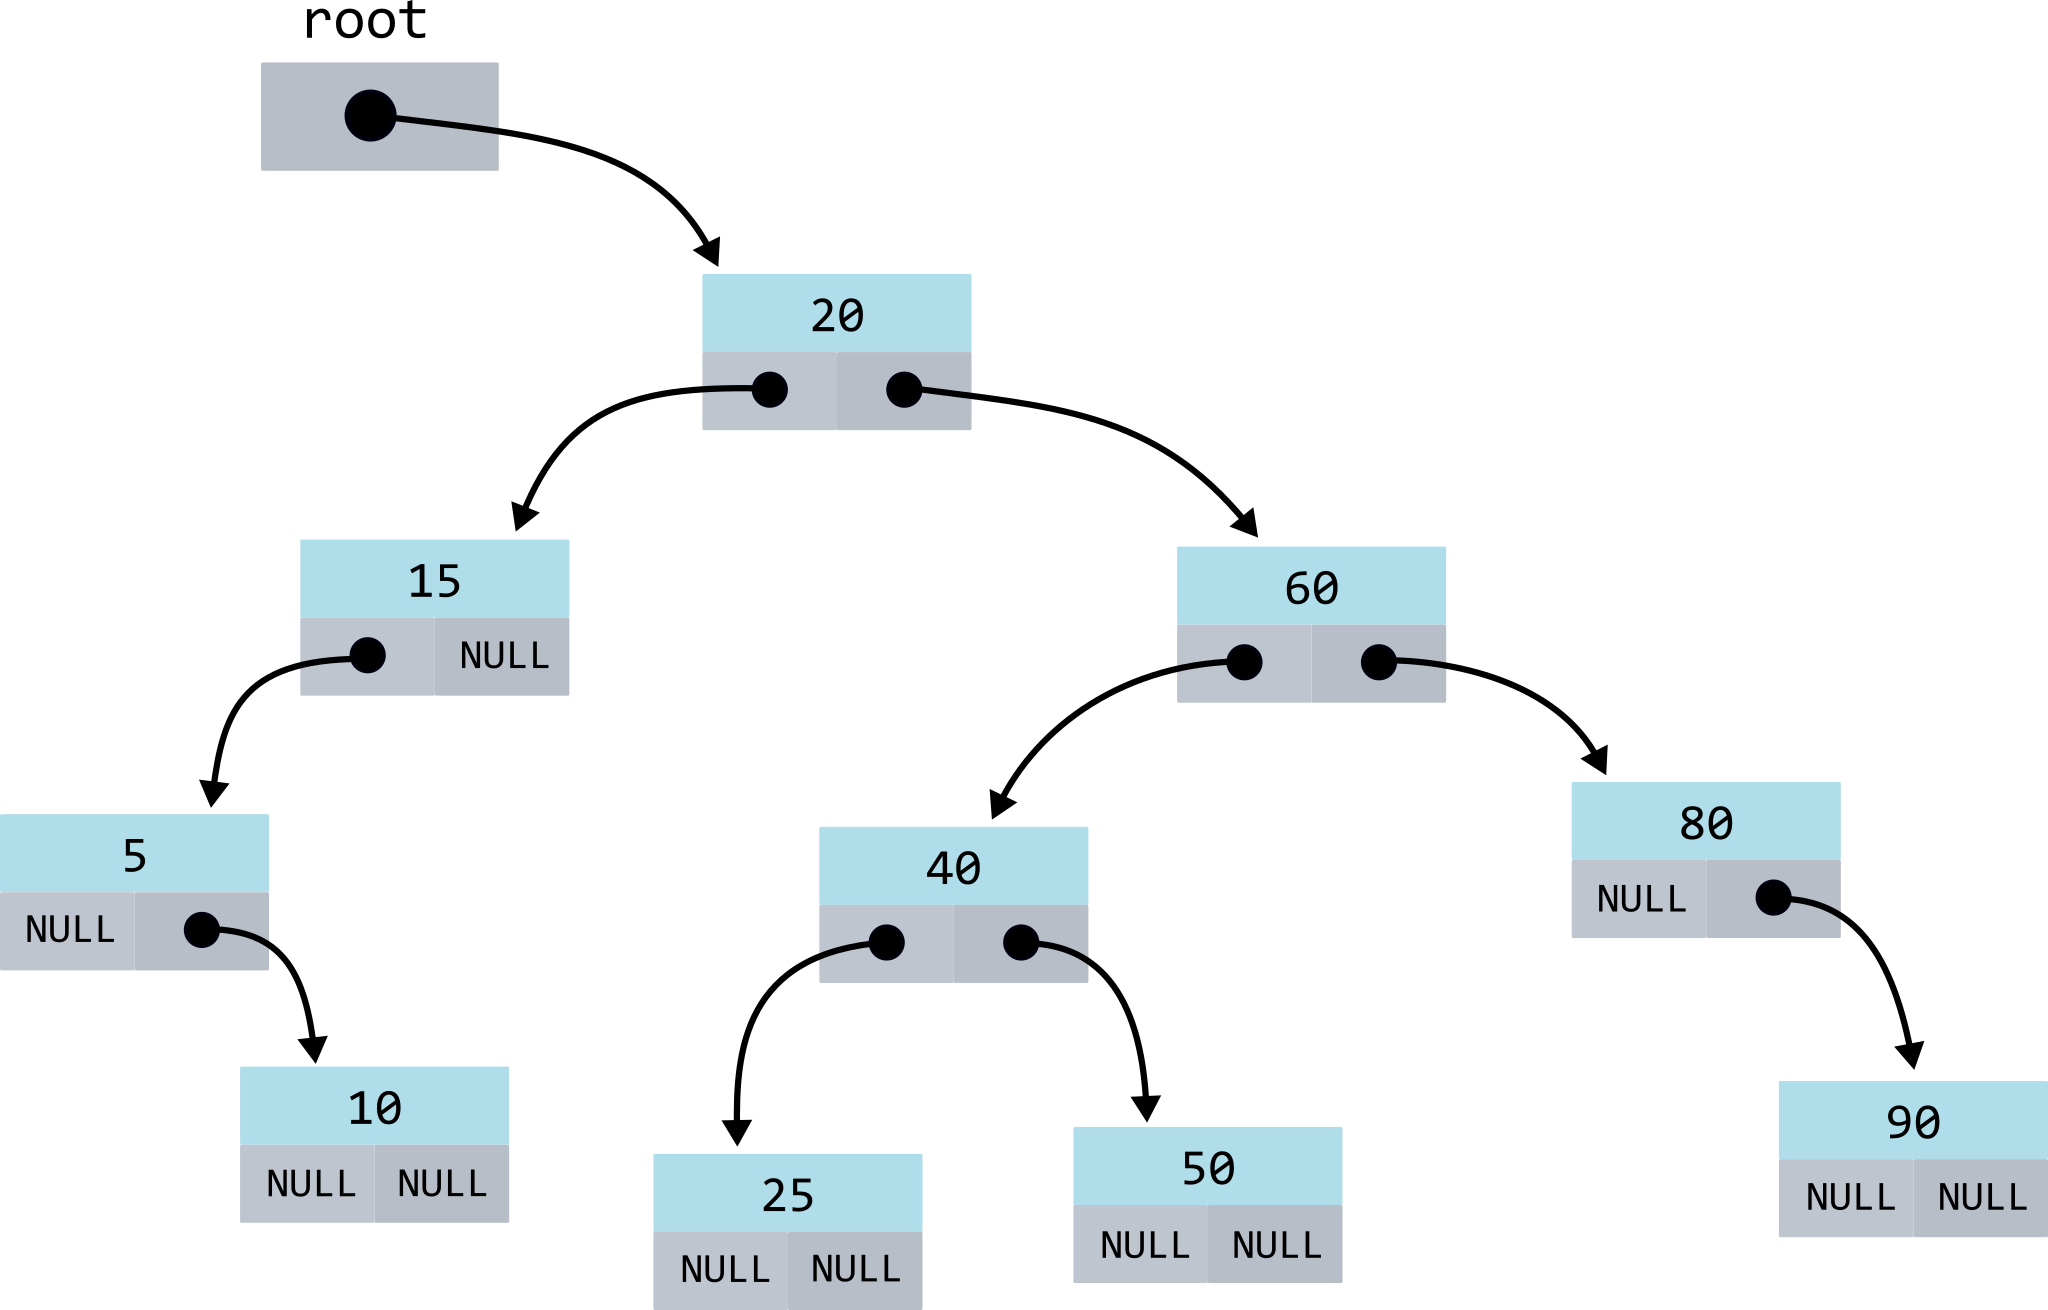
\includegraphics[scale=0.86]{../images/btn.png}
\end{center}

\begin{multicols}{2}
\begin{lstlisting}
struct node {
    int value;
    struct node* left;
    struct node* right;
}
typedef struct node Node;

Node* bst_insert(Node* root, int x) {
  if (root == NULL) {
    root = (Node*)malloc(sizeof(Node));
    root->value = x;
    root->left = NULL;
    root->right = NULL;
  }
  else if (x < root->value)
    root->left = bst_insert(root->left, x);
  else if (x > root->value)
    root->right = bst_insert(root->right, x);
  return root;
}
\end{lstlisting}
\vfill\null
\columnbreak
\textbf{Бинарное дерево} - дерево, в котором у каждого узла может быть не более двух потомков.\\
\textbf{Бинарное дерево поиска (binary search tree -- bst)} - бинарное дерево со следующими условиями:
\begin{itemize}
\item У всех узлов левого поддерева \texttt{value} - меньше
\item У всех узлов правого поддерева \texttt{value} - больше
\end{itemize}
Одинаковые элементы такое дерево не хранит.\\
\textbf{Глубина узла} = количество предков узла + 1\\
\textbf{Высота дерева} = глубина самого глубокого узла\\
Сложность операций с BST:
\begin{itemize}
\item Поиск $O(h(n))$
\item Добавление $O(h(n))$
\item Удаление $O(h(n))$
\end{itemize}
где $h(n)$ - высота дерева.\\
\vfill\null
\end{multicols}
\newpage


Стартовый код для этой части задания в файле \texttt{tree.c}.
\begin{itemize}
\item Написать функцию \texttt{size\_t bst\_size(const Node* root)}, вычисляющую количество элементов в данном дереве. Используйте рекурсию:
\begin{verbatim}
size(корня) = size(левого ребёнка) + size(правого ребёнка) + 1
\end{verbatim}
\item Написать функцию \texttt{size\_t bst\_height(const Node* root)}, вычисляющую глубину бинарного дерева. Используйте рекурсию.
\item Написать функцию \texttt{void bst\_print\_dfs(const Node* root)}, которая будет печатать все элементы дерева в порядке возрастания.
\begin{multicols}{2}
\noindent
\begin{center}
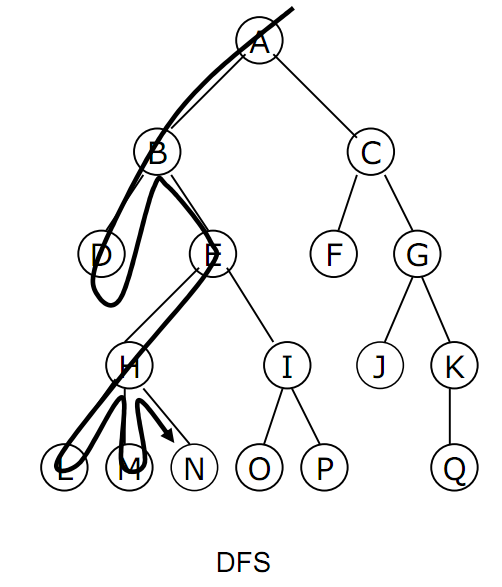
\includegraphics[scale=0.24]{../images/dfs.png}
\end{center}
\columnbreak
\begin{center}
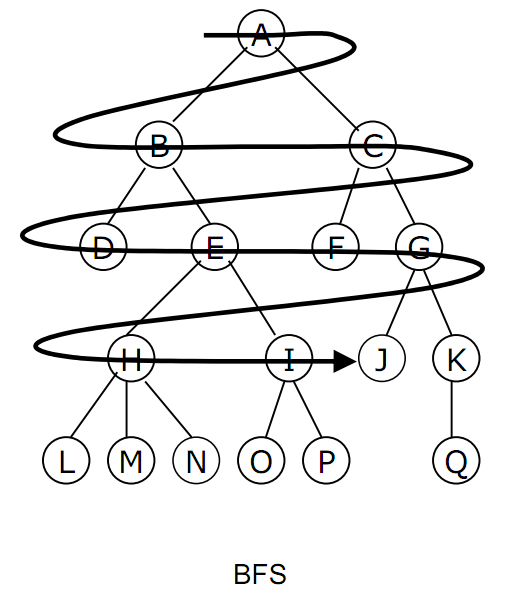
\includegraphics[scale=0.24]{../images/bfs.png}
\end{center}
\end{multicols}
\item Написать функцию \texttt{Node* bst\_search(Node* root, int val)}, которая ищет элемент в бинарном дереве и возвращает указатель на этот элемент. Если такого элемента нет, то функция должна вернуть \texttt{NULL}. Протестируйте эту функцию, печатая поддерево с помощью \texttt{print\_ascii\_tree}.

\item Написать функцию \texttt{Node* bst\_get\_min(Node* root)}, которая возвращает указатель на минимальный элемент в этом дереве.

\item Написать рекурсивную функцию \texttt{Node* bst\_remove(Node* root, int x)}, которая удаляет элемент, содержащий \texttt{x}, из дерева поиска. Функция должна возвращать указатель на узел, который встал на место удалённого узла. Если у удаляемого узла нет детей, то функция должна вернуть \texttt{NULL}.\\
Нужно рассмотреть следующие случаи:
\begin{itemize}
\item Если \texttt{root == NULL}, то ничего не делаем
\item Если \texttt{x > root->value}
\item Если \texttt{x < root->value}
\item Если \texttt{x == root->value} и у \texttt{root} нет детей
\item Если \texttt{x == root->value} и \texttt{root} имеет одного левого ребёнка
\item Если \texttt{x == root->value} и \texttt{root} имеет одного правого ребёнка
\item Если \texttt{x == root->value} и \texttt{root} имеет двух ребёнков. В этом случае делаем следующее:
	\begin{itemize}
	\item Находим минимальный элемент в правом поддереве.
	\item Копируем значение \texttt{val} из этого элемента в \texttt{root}.
	\item Удаляем этот минимальный элемент в правом поддереве, используя функцию \texttt{bst\_remove}.
	\end{itemize}
\end{itemize}
Протестируйте ваш код на всех случаях. Используйте функцию \texttt{print\_ascii\_tree} для проверки.



\item Написать функцию \texttt{void bst\_print\_bfs(const Node* root)}, которая будет печатать элементы в порядке их расстояния от узла (при равенстве расстояния печатать по возрастанию). Тут нужно использовать одну из реализаций абстрактного типа данных Очередь.
\end{itemize}
\newpage
\section*{Часть 2: Сбалансированные деревья} 
Сбалансированное дерево -- это дерево у которого для \textit{каждого} узла высоты левого поддерева и правого различаются не более, чем на 1.
\begin{multicols}{2}

\textbf{Пример 1:}\\

Это дерево сбалансированное. Так как для узла \texttt{A} глубины левого и правого поддерева равны.
Для узлов \texttt{B} и \texttt{C} глубины левого и правого поддерева отличается всего на \texttt{1} 
(глубина левого поддерева равна 1, а глубина правого равна нулю).

\begin{center}
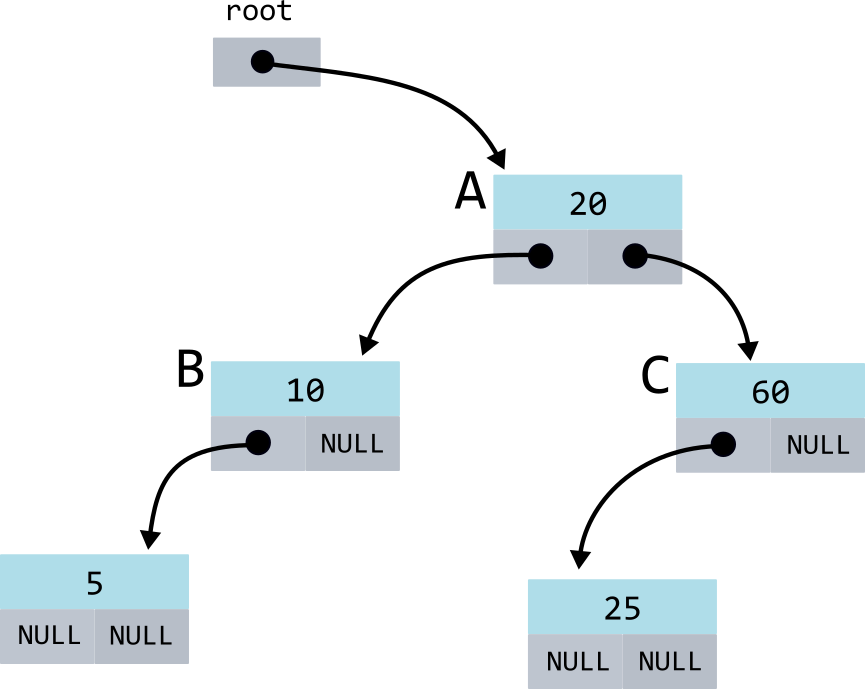
\includegraphics[scale=0.8]{../images/balanced_tree.png}
\end{center}
\vfill\null
\columnbreak

\textbf{Пример 2:} \\

Это дерево несбалансированное. Так как уже у корня дерева, высота левого поддерева равна 2, а высота правого поддерева равна 5. Разница высот больше, чем 1.
\begin{center}
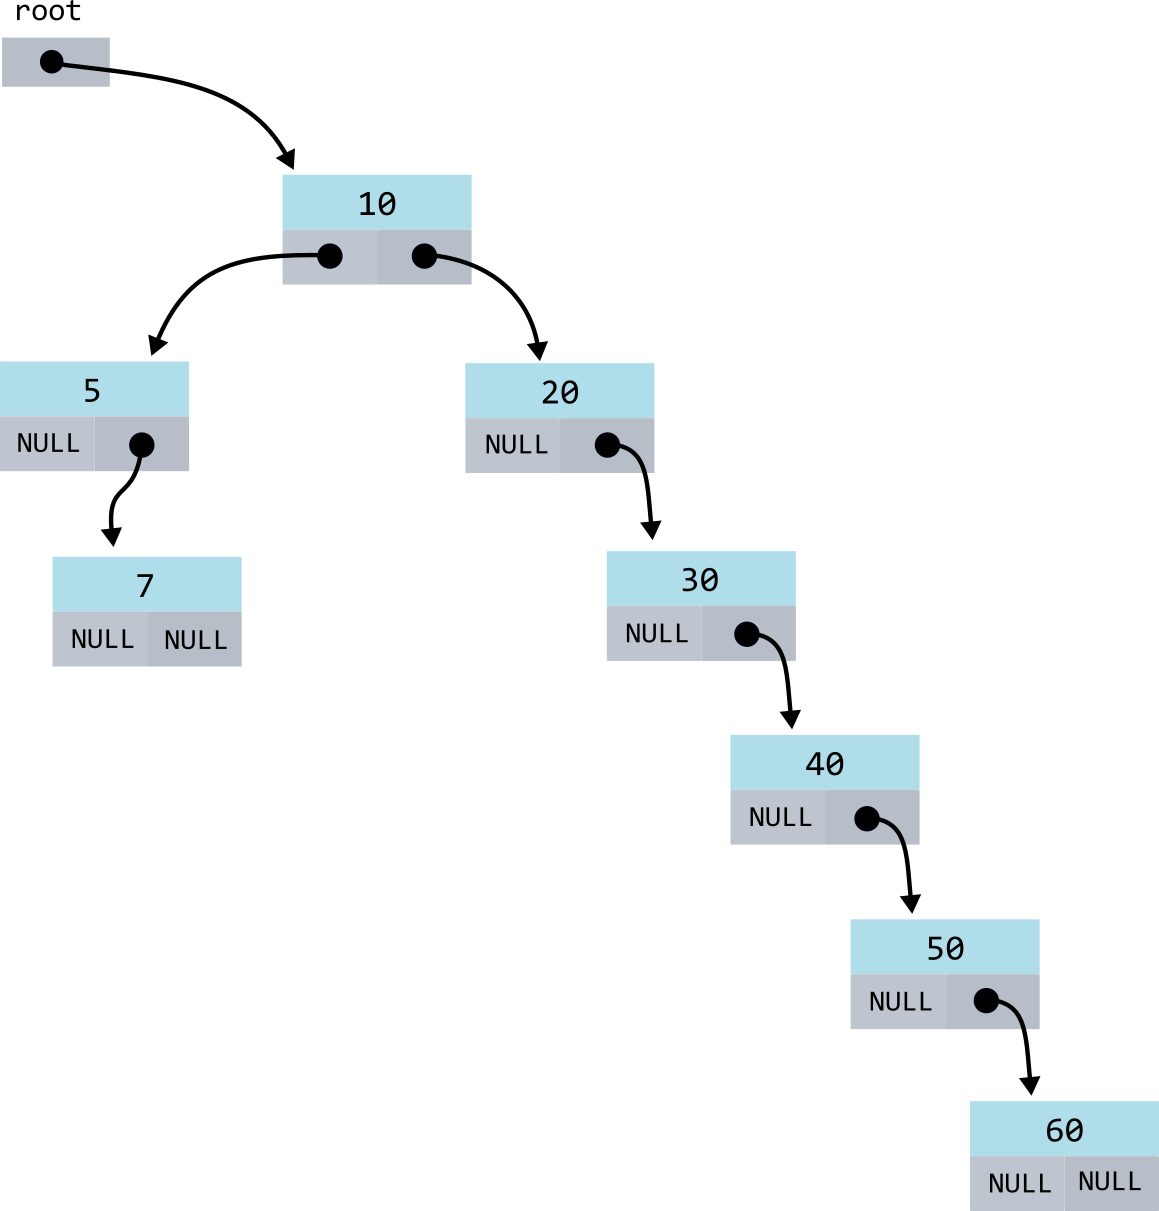
\includegraphics[scale=0.9]{../images/unbalanced_tree.png}
\end{center}
\end{multicols}

Можно показать, что для любого сбалансированного дерева его высота пропорциональна логарифму количества элементов и, как следствие, $h(n) = O(\log(n))$. Для несбалансированных деревьев высота может быть намного больше чем $\log(n)$. В худшем случае дерево вырождается в связный список.

Так как вычислительная сложность операций с деревом зависит от высоты дерева, то нам очень важно, чтобы дерево было сбалансированным. В ином случае, операции поиска/добавления/удаления будут работать намного медленнее. К сожалению, обычное бинарное дерево поиска, написанное нами в предыдущей части, не является сбалансированным. Это можно понять, если представить, что будет при добавлении в дерево последовательно возврастающих элементов с помощью функции \texttt{bst\_insert}.\\

Однако, можно модифицировать бинарное дерево поиска так, чтобы дерево всегда оставалось сбалансированным. Есть два основных способа такой модификации:
\begin{enumerate}
\item AVL-деревья
\item Красно-черные деревья
\end{enumerate}
Для самобалансирующихся деревьев поиска гарантируется, что вычислительная сложноть основных операций с ними будет равна $O(\log(n))$.

\subsection*{Задачи:}
\begin{itemize}
\item Заполнить дерево $n = 20000$ случайных чисел и найти количество элементов и высоту этого дерева. Сравнить высоту с оптимальной $h_{optimal} = \ceil*{log_2(n + 1)} = 14.3$. Помните, что вычислительная сложность операций с деревом равна $O(h)$, где $h$ -- высота дерева.
\item Заполнить дерево  $n = 20000$ последовательными числами и найти количество элементов и высоту такого дерева. Сравнить высоту с оптимальной. Что будет, если увеличить $n$ до миллиона?
\end{itemize}


\section*{Часть 3: AVL-дерево (самобалансирующееся дерево поиска)} 
Основная идея самобалансирующихся деревьев, заключается в следующем:
\begin{enumerate}
\item Считаем, что дерево сбалансированное
\item После каждой вставки элемента в дерево проверям, нарушилась ли балансировка дерева. То есть не появился ли у нас узел, для которого высоты левого и правого поддеревьев различаются более чем на 1.
\item Если такой узел появился, то перенаправляем указатели соседних узлов так, чтобы дерево стало вновь сбалансированным.
\end{enumerate}

Чтобы не вычислять при каждой вставке высоту узла, будем хранить ей в узле (поле \texttt{height}):
\begin{lstlisting}
struct node {
    int value;
    int height;
    struct node* left;
    struct node* right;
};
typedef struct node Node;
\end{lstlisting}

\newpage
\subsection*{Пример самобалансирования \texttt{AVL}-дерева}

\begin{center}
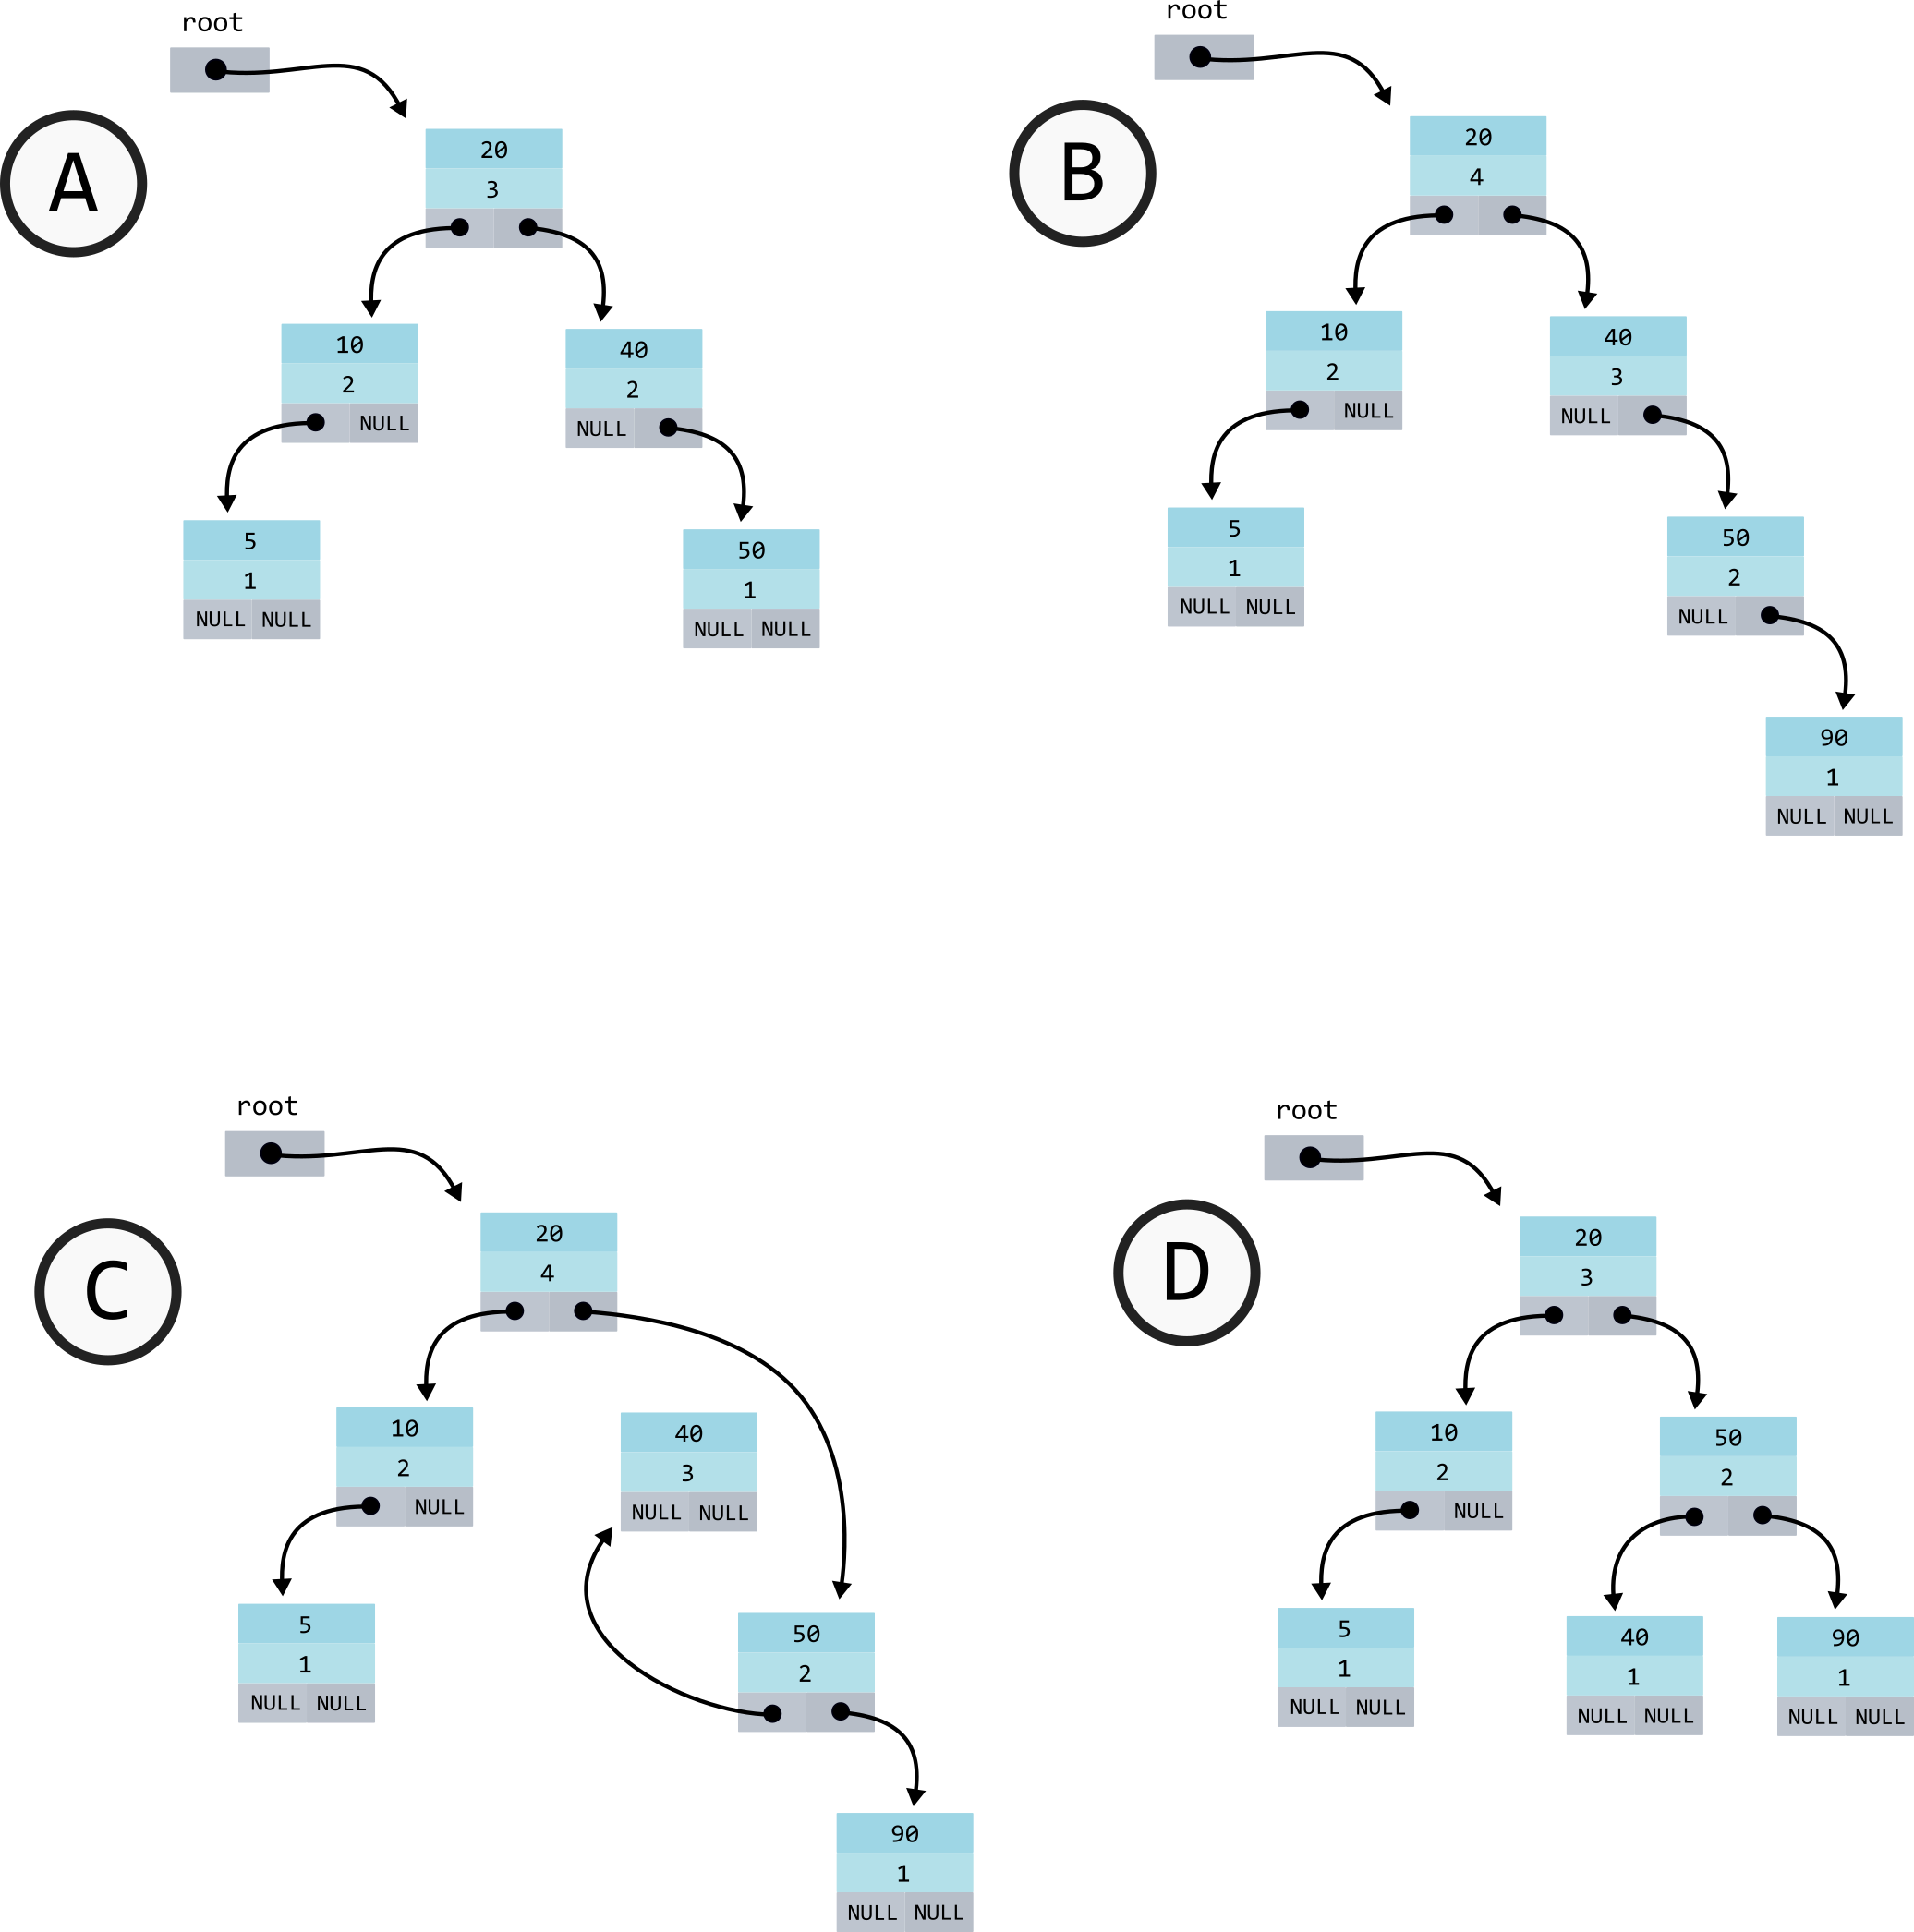
\includegraphics[scale=0.9]{../images/avl_example.png}
\end{center}

\begin{enumerate}
\item[A:] Вначале дерево сбалансированно
\item[B:] Затем мы добавляем один элемент и дерево перестаёт быть сбалансированным. Так как для узла, хранящего значение \texttt{40} высота левого поддерева равна \texttt{0}, а высота правого поддерева равна \texttt{2}.
\item[C:] Затем, мы перенаправляем указатели у соседних узлов так, чтобы условие сбалансированности дерева вновь начало соблюдаться.
\item[D:] В конце просто корректируем значения высот для поддеревьев.
\end{enumerate}

\subsection*{Задачи:}
\begin{itemize}
\item Рассмотрите случай, когда в дерево \texttt{A} добавляют элемент, равный \texttt{1}. Как нужно перенаправить указатели в этом случае?
\item Рассмотрите случай, когда из дерева \texttt{A} сначала удаляют элемент, равный \texttt{5}, а потом добавляют элемент, равный \texttt{90}. Как нужно перенаправить указатели в этом случае?
\item Рассмотрите случай, когда из дерева \texttt{A} сначала удаляют элемент, равный \texttt{5}, а потом добавляют элемент, равный \texttt{30} и затем добавляют элемент, равный \texttt{25}. Как нужно перенаправить указатели в этом случае?
\end{itemize}


\iffalse
\newpage
\section*{AVL-деревья}

\begin{lstlisting}
struct node {
    int val;
    struct node* left;
    struct node* right;
    int height;
};
typedef struct node Node;
\end{lstlisting}
Стартовый код для этой части задания в файле \texttt{avl.c}.
\begin{itemize}
\item Написать функцию \texttt{void left\_rotate(Node** proot)}. Проверьте функцию, используя \texttt{print\_ascii\_tree}.
\item Написать функцию \texttt{void right\_rotate(Node** proot)}
\begin{multicols}{2}
\noindent
\begin{lstlisting}
         левое вращение

       x                 y     
      / \     LR(x)     / \     
     A   y     =>      x   C    
        / \           / \       
       B   C         A   B      

         правое вращение
   
        y              x 
       / \    RR(y)   / \
      x   C    =>    A   y
     / \                / \
    A   B              B   C
\end{lstlisting}
\end{multicols}
Тут \texttt{x} и \texttt{y} - узлы, а \texttt{A}, \texttt{B} и \texttt{С} - произвольные поддеревья.
\item Написать функцию \texttt{void rebalance(Node** proot)}. Тут нужно рассмотреть 4 случая. 
\begin{itemize}
\item Если самая длинная ветвь справа-справа, то нужно сделать \texttt{LR(x)}.
\begin{lstlisting}
       
  x                      y                  
 / \                    / \                  
A   y       LR(x)      x   z                 
   / \       =>       / \  /\                        
  B   z              A  B C  D                          
     / \                                        
    C   D                                         
\end{lstlisting}
\item Если самая длинная ветвь справа-слева, то нужно сделать \texttt{RR(z)} и \texttt{LR(x)}.
\begin{lstlisting}
       
       x                 x                      y                  
      / \               / \                    / \                  
     A   z     RR(z)   A   y       LR(x)      x   z                 
        / \     =>        / \       =>       / \  /\                        
       y   D             B   z              A  B C  D                          
      / \                   / \                                        
     B   C                 C   D                                         
\end{lstlisting}
\item Два других случая для левой ветви зеркально симметричны.
\end{itemize}

\item Написать функцию \texttt{tree\_fix\_height(Node* root)}, которая будет вычислять высоту узла \texttt{root}, при условии, что поле \texttt{height} у его детей задано правильно. Её нужно вызывать при каждом изменении дерева.
\item Заполнить AVL-дерево миллионом случайных чисел и найти количество элементов и высоту этого AVL-дерева. Сравнить высоту с оптимальной.
\item Заполнить AVL-дерево миллионом последовательный чисел (от $1$ до $10^6$) и найти количество элементов и высоту этого AVL-дерева. Сравнить высоту с оптимальной.
\end{itemize}
\fi
\end{document}
